\section{Task Analysis}
\label{sec:task}
Identify the analysis goals and the corresponding visualization tasks is the first yet significant step in designing a useful tool. In this section, we first examine how domain experts normally approach the task of analyzing a model (i.e., assess its strength and weakness) and identify where and how an interactive visualization system can aid in such a process.
% and how they fit into the domain experts experts' though process and workflow.
Then, we reify the observations into concrete goals, from which we identify the visualization tasks that guide the design and implementation of the proposed tool.

During our long-term collaboration with NLP experts, we have conducted extensive interview and discussion on the common approach employed by research for assessing the behavior of a model.%
The prediction accuracy has it place as an objective evaluation metric to measure the overall effectiveness of the model, however, the accuracy number alone does not provide the full story. For example, the model can perform much worse on a different test set, or the model may produce correct predictions for the ``wrong'' reasons (e.g., pickup unintended pattern in the training data that does not exist in real word scenarios).
%
Therefore, beside standard metrics, the domain experts often rely on exploration centric approach to 
conduct error analysis and obtain intuition.
%
Such a process is iterative in nature, in which the domain experts go through many cycles of examine examples (e.g, what are the mistakes made by the model), and conduct experiments (e.g., perturb the input and observe the changes), formulate hypothesis (e.g, what are the potential causes for the failure).
%ultimate forms intuition about the strength or the weakness of a given model. 
% , then additional examples or variation of existing examples are bring in to rejected or confirm the hypotheses. And new questions or hypothesis may arise.
%Such an analysis is iterative in nature and guided by domain knowledge and hypotheses based on the architecture. As they ask more questions and experiment 
%experiment with model iterate their understanding of the model behavior, ultimate forms intuition about the strength or the weakness of a given model. 
%and come up hypothesis about the potential cause for the failure. 

%%% iterative process call for interactive visualization

%
A stereotypical scenario can be summarized as the follow.
To assess a model for a specific NLP task, the research start the analysis by looking at the failure cases.
Look at example, perturb the example, see how the perturb the one fails,
learn the limitation and strength from the where and how the errors occurs. iterate 


%\begin{figure}[htbp]
%\centering
%\vspace{-2mm}
% 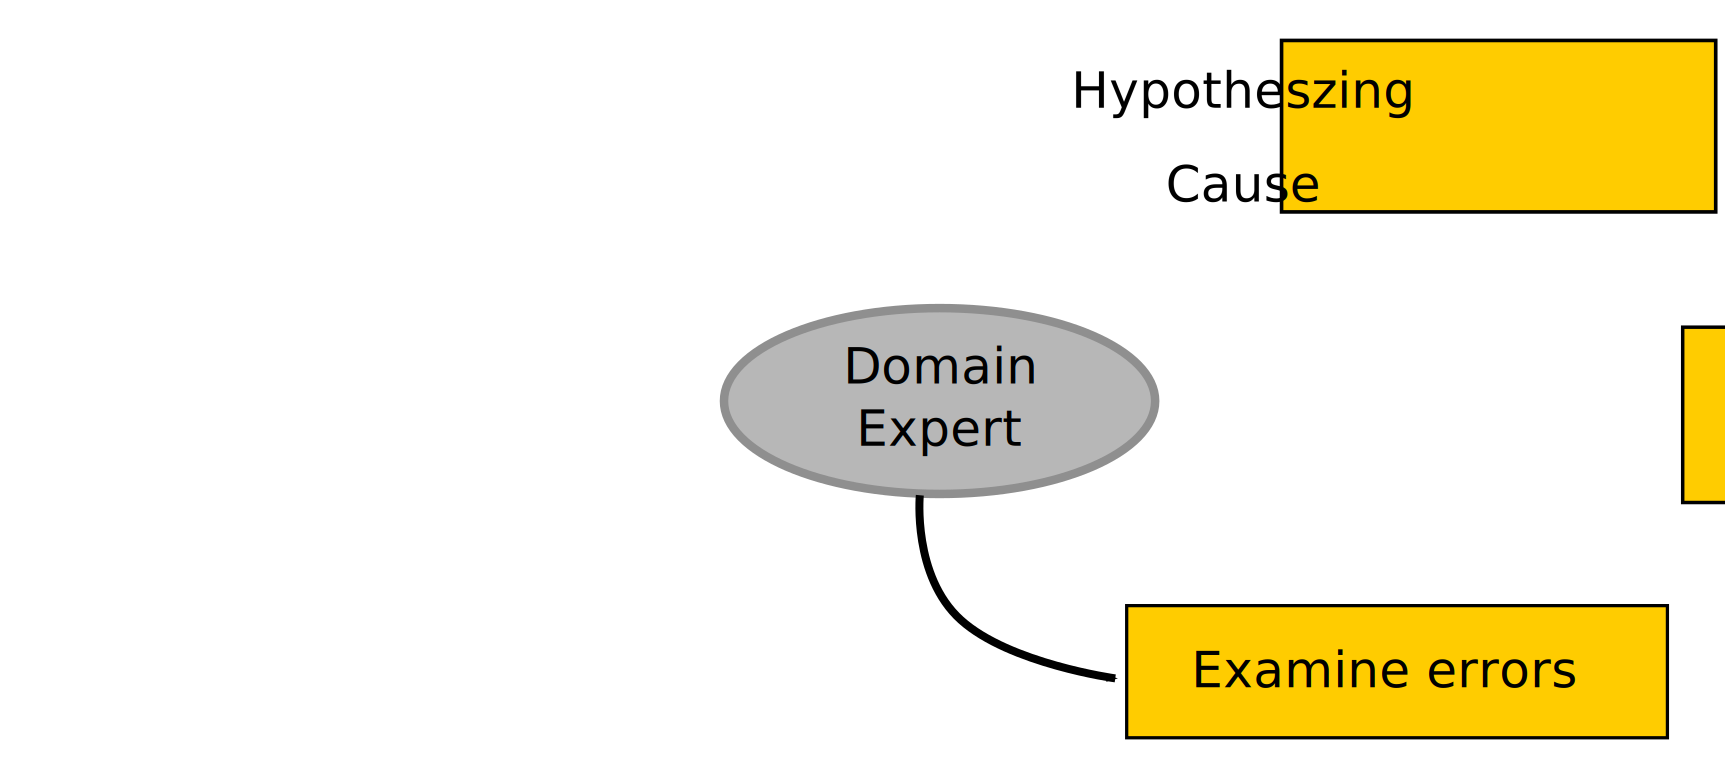
\includegraphics[width=1.0\linewidth]{errorAnalysis}
% \caption{How domain experts conduct error analysis on the model.}
%\label{fig:modelPipeline}
%\end{figure}

Analysis Goal
\begin{itemize}
\item \textbf{G1} Understand how attention affect the prediction 
\item \textbf{G2} Why sentences are misclassified 
\item \textbf{G3} 
\item \textbf{G4} 
\end{itemize}

Visualization Tasks
\begin{itemize}
\item \textbf{T1} Encode the internal state \emph{attention} of the model
\end{itemize}
